%----------------------------------------------------------------------------------------
%	PACKAGES AND OTHER DOCUMENT CONFIGURATIONS
%----------------------------------------------------------------------------------------

\documentclass[twoside,twocolumn,a4paper]{article}

\usepackage{blindtext} % Package to generate dummy text throughout this template 

\usepackage{mhchem}

\usepackage{gensymb}

%\usepackage[super]{natbib}

\usepackage[T1]{fontenc} % Use 8-bit encoding that has 256 glyphs

\usepackage{lmodern}

\usepackage[hyphenbreaks]{breakurl}

\usepackage[hyphens]{url}

%\usepackage[super,sort&compress]{natbib}
%\usepackage{natbib}
%\setlength{\bibsep}{0.0pt}

\usepackage{graphicx}

\linespread{1.05} % Line spacing - Palatino needs more space between lines
\usepackage{microtype} % Slightly tweak font spacing for aesthetics

\usepackage[spanish]{babel} % Language hyphenation and typographical rules

\usepackage[numbib,notlof,notlot,nottoc]{tocbibind} % Shows bibliography as a section

\usepackage[hmarginratio=1:1,top=32mm,columnsep=20pt]{geometry} % Document margins

\usepackage[hang, small,labelfont=bf,up,textfont=up]{caption} % Custom captions under/above floats in tables or figures

\usepackage[section]{placeins}

\usepackage{float}

\usepackage{booktabs} % Horizontal rules in tables

\usepackage{enumitem} % Customized lists

\setlist[itemize]{noitemsep} % Make itemize lists more compact

\usepackage{abstract} % Allows abstract customization

\renewcommand{\abstractnamefont}{\normalfont\bfseries} % Set the "Abstract" text to bold

\usepackage{fancyhdr} % Headers and footers
\pagestyle{fancy} % All pages have headers and footers
\fancyhead{} % Blank out the default header
\fancyfoot{} % Blank out the default footer
\fancyhead[C]{Laboratorio 4 $\bullet$ Informe Pr\'actica Especial $\bullet$ Grupo 3: Poggi, R\'ios Ch\'avez} % Custom header text
\fancyfoot[C]{\thepage} % Custom footer text

\usepackage{titling} % Customizing the title section

\usepackage{hyperref} % For hyperlinks in the PDF

%----------------------------------------------------------------------------------------
%	TITLE SECTION
%----------------------------------------------------------------------------------------

\setlength{\droptitle}{-4\baselineskip} % Move the title up

\pretitle{\begin{center}\LARGE\bfseries} % Article title formatting
\posttitle{\end{center}} % Article title closing formatting
\title{Caracterizaci\'on de una celda Peltier} % Article title
\author{%
\textsc{Ignacio Poggi} \\[1ex] % Your name
\normalsize \href{mailto:ignaciop.3@gmail.com}{ignaciop.3@gmail.com} % Your email address
\and % Uncomment if 2 authors are required, duplicate these 4 lines if more
\textsc{Carlos R\'ios Ch\'avez} \\[1ex] % Second author's name
\normalsize \href{mailto:carlos_rios_ch@hotmail.com}{carlos\_rios\_ch@hotmail.com} % Second author's email address
}



\date{Grupo 3 - Laboratorio 4, C\'atedra Schmiegelow - Departamento de F\'isica, Facultad de Ciencias Exactas y Naturales, Universidad de Buenos Aires \newline \\ \today} % Leave empty to omit a date
\renewcommand{\maketitlehookd}{%
\begin{abstract}
\noindent En este trabajo se realiz\'o la caracterizaci\'on de una celda Peltier midiendo el coeficiente de Seebeck $\alpha$, resistencia $R$ y conductividad t\'ermica $K$; a trav\'es de los datos obtenidos de la diferencia de temperatura, voltaje y corriente circundante entre sus dos caras. Finalmente se obtuvo el rendimiento de la celda y se compar\'o con el de otras m\'aquinas t\'ermicas.
\end{abstract}
}

%----------------------------------------------------------------------------------------

\begin{document}
\maketitle

% Print the title

%----------------------------------------------------------------------------------------
%	ARTICLE CONTENTS
%----------------------------------------------------------------------------------------

\section{Introducci\'on}


Se denomina termoelectricidad a un conjunto de efectos o fen\'omenos f\'isicos que relacionan a la termodin\'amica con la electricidad. En equilibrio termodin\'amico, los portadores de carga en un conductor pueden generar un flujo de calor, pudiendo transformar energ\'ia mec\'anica en energ\'ia t\'ermica y viceversa. Entre estos fen\'omenos, podemos destacar el efecto Seebeck, Peltier y Joule.

\subsection{Efecto Seebeck}

Si se tiene un circuito formado por dos metales distintos, $A$ y $B$, con dos uniones a diferente temperatura, $T$ y $T + \Delta T$, se establece un flujo de corriente el\'ectrica debido a que los portadores de carga difunden en contra del gradiente de temperatura. Esto produce acumulaci\'on de carga en el extremo fr\'io y un vaciamiento del extremo caliente del termopar. Este desbalance de portadores genera un campo el\'ectrico, que a su vez origina una fuerza termoelectromotriz $\epsilon_{AB}$, que depende de los metales utilizados en la uni\'on y de la diferencia de temperatura entre las dos uniones.\\

Se puede definir al coeficiente Seebeck $\alpha_{AB}$ como la relaci\'on entre $\epsilon_{AB}$ y $T$, de la siguiente manera [1]:

\begin{equation}
\label{eq:seebeck}
\alpha_{AB} = \frac{d\epsilon_{AB}}{dT}
\end{equation}

La ecuaci\'on (\ref{eq:seebeck}) puede definirse en t\'erminos de la diferencia de potencial $\Delta V$ como:

\begin{equation}
\label{eq:seebeck2}
\alpha_{AB} = \frac{\Delta V}{\Delta T}
\end{equation}

donde $\Delta V$ y $\Delta T$ son las diferencia de potencial neta  y temperatura entre los metales $A$ y $B$, respectivamente.

\subsection{Efecto Peltier}

Rec\'iprocamente al efecto Seebeck, al circular una corriente el\'ectrica $I$ por la uni\'on entre distintos materiales, se produce una transferencia de calor, como se esquematiza en la Figura \ref{fig:peltier}. La potencia calor\'ifica intercambiada en la uni\'on entre los puntos $A$ y $B$ es [2]:

\begin{equation}
\label{eq:peltier}
\dot{Q} = J\Delta T \alpha_{AB} = J \pi_{AB}
\end{equation}

siendo $\pi_{AB}$ el coeficiente Peltier (calor intercambiado en la uni\'on por unidad de tiempo y de corriente que circula por la misma), $J$ el flujo de corriente el\'ectrica, $\Delta T$ la diferencia de temperatura entre los puntos $A$ y $B$, y $\alpha_{AB}$ el coeficiente Seebeck.


\begin{figure}[H]
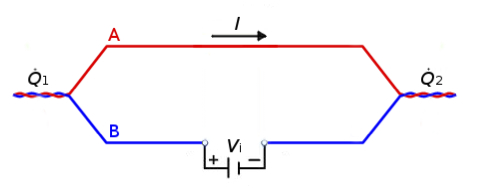
\includegraphics[width=\linewidth]{peltier.jpg}
\caption{Esquema de un circuito formado por los materiales A y B con dos uniones. La circulaci\'on de corriente origina un flujo de calor, produciendo el efecto Peltier.}
\label{fig:peltier}
\end{figure}

\subsection{Efecto Joule}

Para una caracterizaci\'on completa de la celda, se deben tener en cuenta la difusi\'on de calor a trav\'es de la misma debido al gradiente de temperatura, y la disipaci\'on por efecto Joule.\newline

\par
La difusion de calor del lado mas caliente al fr\'io por unidad de tiempo para cada elemento esta dado por la ley de Fourier [3]:

\begin{equation}
\label{eq:calor}
\dot{Q}_{Fourier} = -k \frac{A}{L} \Delta T
\end{equation}

donde $k$ es el coeficiente de conductividad t\'ermica de cada elemento por unidad de longitud, $A$ el \'area, $l$ la longitud de cada elemento y $\Delta T$ la diferencia de temperatura en los extremos (el signo negativo indica que el calor fluye en contra del gradiente de temperatura).\newline

\par
El efecto Joule est\'a representado por la transformaci\'on de trabajo el\'ectrico en calor, debido a la resistencia $R$ del circuito. La p\'erdida de energ\'ia asociada es [4]:

\begin{equation}
\label{eq:joule}
\dot{Q}_{Joule} = I^{2}R = I^{2}\rho \frac{L}{A}
\end{equation}

donde $\rho$ es la resistividad el\'ectrica del conductor respectivamente.


\subsection{Celdas termoel\'ectricas}

Una celda Peltier est\'a compuesta por un cierto n\'umero de termopares (pares de semiconductores de tipo N y P), conectados en serie con las uniones ubicadas alternadamente sobre las dos caras. Dichas caras est\'an recubiertas de un material cer\'amico, para mejorar la disipaci\'on del calor, como muestra la Figura \ref{fig:celda}.

\begin{figure}[H]
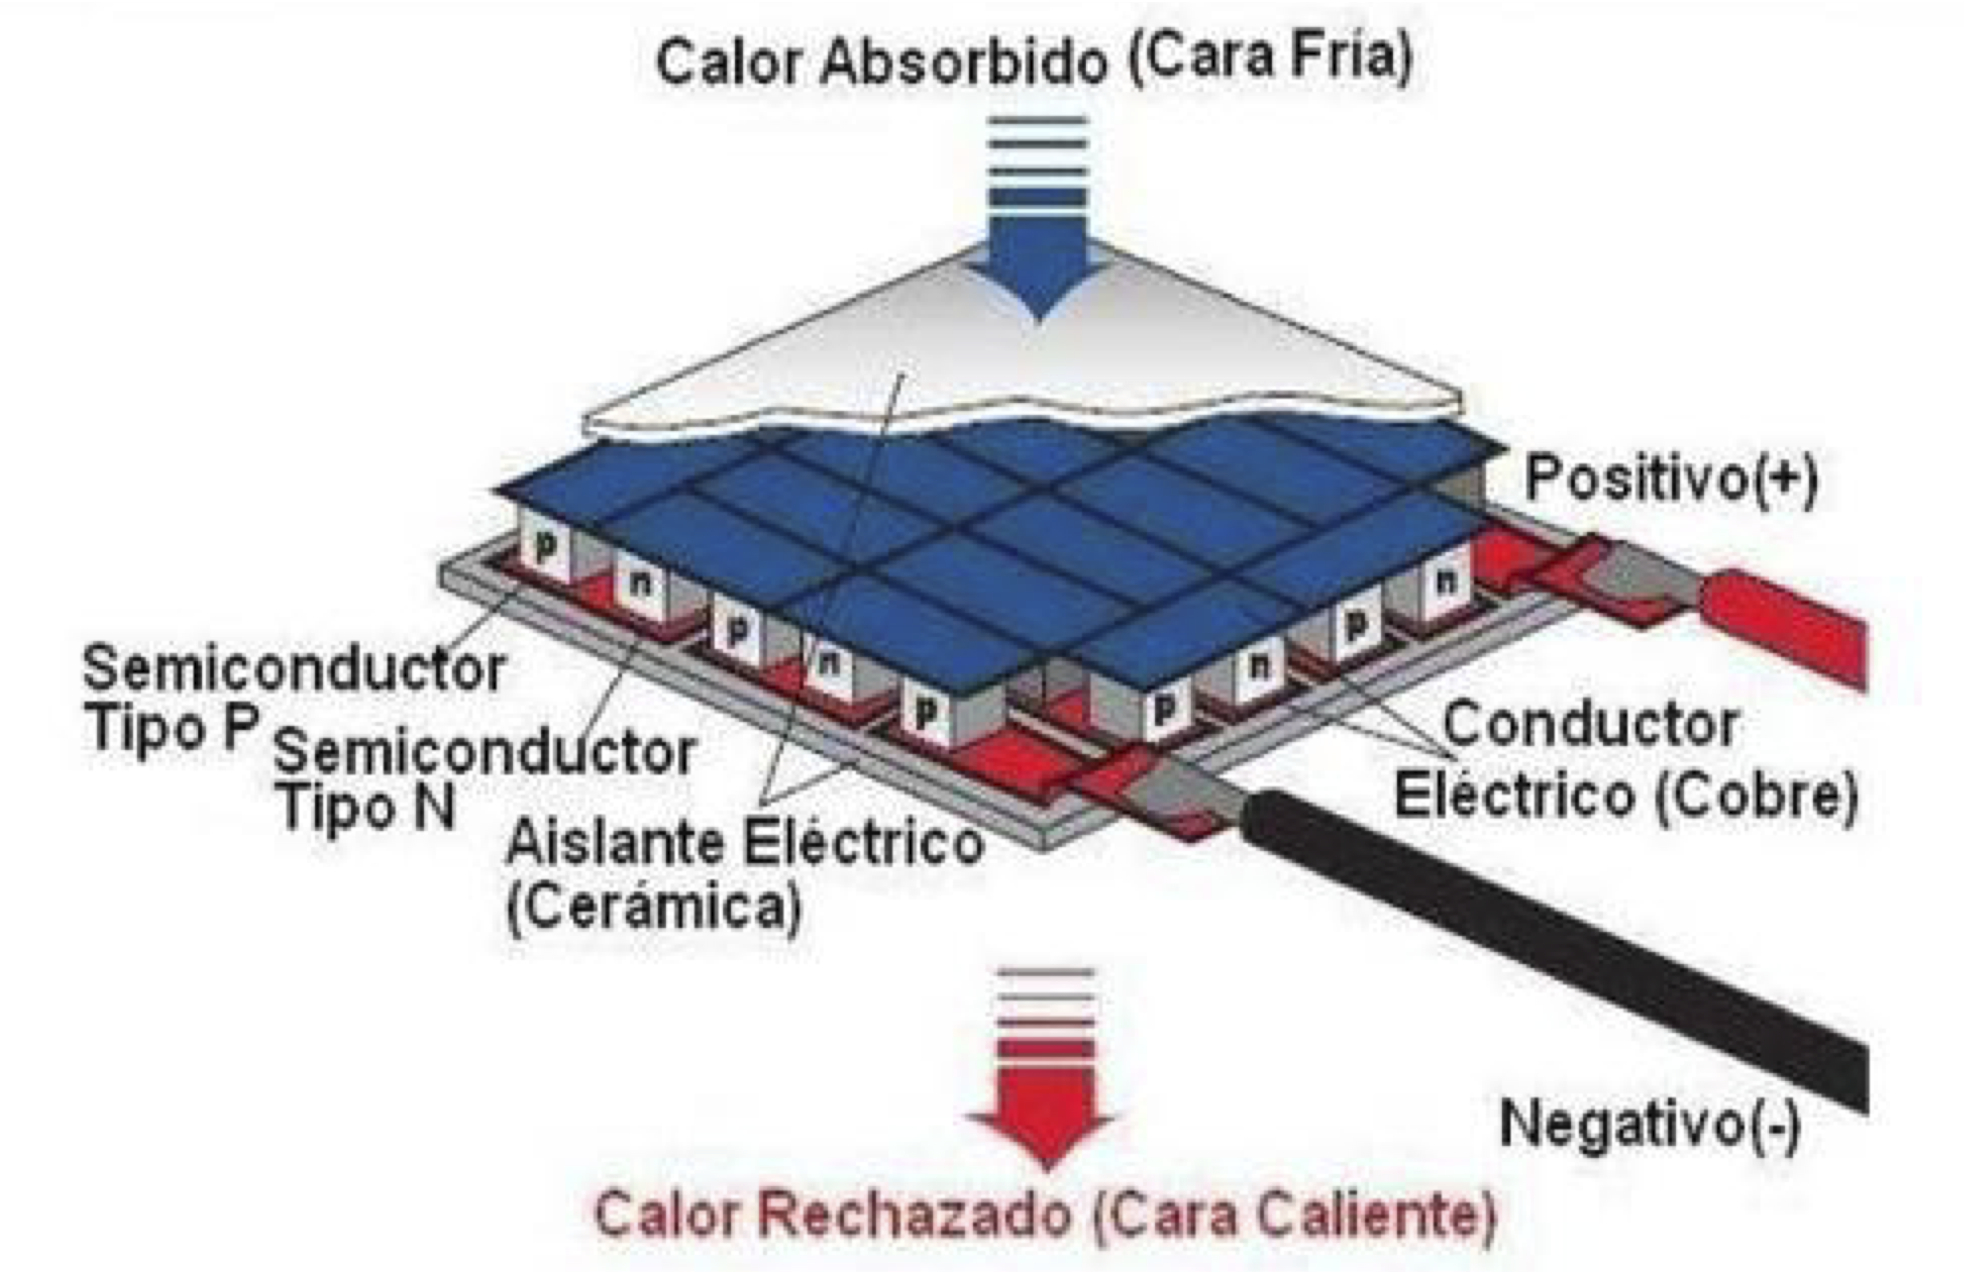
\includegraphics[width=\linewidth]{celda.jpg}
\caption{Esquema de una celda Peltier. Se observan los componentes semiconductores en el interior de la misma y las caras cer\'amicas a distinta temperatura.}
\label{fig:celda}
\end{figure}

Si ambas caras de la celda se encuentran en contacto con reservorios a distintas temperaturas, se manifiesta el efecto Seebeck, por lo tanto puede ser utilizada como generador de electricidad. An\'alogamente, al hacer pasar una corriente $I$ por la misma, las uniones sobre una de las caras absorber\'an y las contrarias liberar\'an calor (efecto Peltier), operando como una m\'aquina frigor\'ifica o una fuente de calor.\\

Por \'ultimo, para calcular el rendimiento de la celda como maquina termica, utilizando las ecuaciones (\ref{eq:peltier}) y (\ref{eq:joule}) se obtiene que el calor intercambiado en cada una de las caras (en r\'egimen estacionario) es [5]:

\begin{equation}
\label{eq:qcaras}
\dot{Q_{i}} = \pm I\alpha T_{i} - K(T_{i} - T_{j}) + \frac{I^{2}R}{2}
\end{equation}


donde $\alpha$ y $K$ contienen la contribuci\'on de todos los elementos conductores al efecto Peltier y a la difusi\'on de calor, y $i = \{1,2\}$. De la misma forma, la potencia el\'ectrica aplicada esta dada por la siguiente ecuaci\'on [6]:

\begin{equation}
\label{eq:potencia}
\dot{W} = VI = I \alpha \Delta T + I^{2}R
\end{equation}

Mediante las ecuaciones (\ref{eq:qcaras}) y (\ref{eq:potencia}), se puede obtener la eficiencia y el rendimiento de la celda como m\'aquina t\'ermica con las siguientes expresiones:


\begin{equation}
\label{eq:eficiencia}
\eta = \frac{-\dot{W}}{-\dot{Q_{c}}}
\end{equation}

\begin{equation}
\label{eq:rendimiento}
COP = \frac{-\dot{Q_{f}}}{+\dot{W}}
\end{equation}

siendo $\dot{Q_{f}}$ y $\dot{Q_{c}}$ el calor intercambiado por la cara fria y caliente, respectivamente.



%------------------------------------------------

\section{Dispositivo experimental}

El primer armado experimental consisti\'o en una celda Peltier; en cada una de sus caras se ubicaron dos sensores de temperatura LM-35 alimentados con 7,5 V mediante un generador de corriente continua LG GP4303D. Estos estaban dentro de un hueco en dos cubos de aluminio que actuaban como disipador de calor. La celda fue alimentada con el generador de corriente continua Agilent B2901A, el cual tambi\'en permiti\'o la obtenci\'on del voltaje y corriente circulando por el circuito compuesto por la celda.\\

A su vez, se tomaron las mediciones de los sensores LM-35 a trav\'es de la placa de adquisici\'on de datos National Instruments NI-USB 6120 hacia una PC con MATLAB; lo que permiti\'o determinar la temperatura de cada sensor. La relaci\'on entre voltaje de salida y temperatura medida en cada uno de ellos es de 10 mV/\degree C, su rango de medici\'on es de -55 \degree C (-550 mV) a 150 \degree C (1500 mV) y la precisi\'on a temperatura ambiente es de 0,5 \degree C. En la siguiente figura se muestra un esquema del dispositivo utilizado:

\begin{figure}[H]
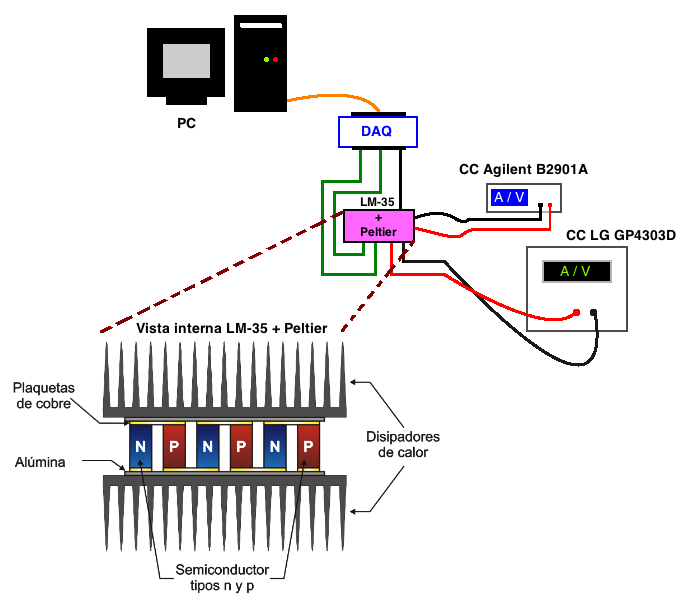
\includegraphics[width=\linewidth]{dispexp.jpg}
\caption{Esquema del primer dispositivo experimental utilizado. Se puede apreciar el detalle del armado interno donde se encuentra ubicada la celda Peltier.}
\label{fig:dispexp}
\end{figure}

Los datos obtenidos en esta primera parte (voltaje, corriente y temperaturas) permitieron obtener la evoluci\'on de la temperatura en funci\'on del tiempo y el coeficiente de Seebeck $\alpha$.\\

Finalmente, para obtener el rendimiento como m\'aquina frigor\'ifica, la conductividad t\'ermica $K$ y la resistencia $R$ de la celda Peltier, se calcul\'o la potencia entregada a la misma y la absorbida por la cara fr\'ia. La primera se obtuvo como la corriente circulante por la tensi\'on entre las placas (la cara caliente de la celda se ubic\'o sobre un bloque de hierro para que est\'e a temperatura constante) y para la segunda se coloc\'o un disipador de aluminio con un sensor de temperatura LM-35 sobre la cara fr\'ia (todo el conjunto encerrado en un termo de aluminio), pudiendo obtener el cambio de temperatura en el tiempo de la misma a trav\'es de la placa de adquisici\'on. En la siguiente figura se esquematiza el armado experimental para esta parte del trabajo:

\begin{figure}[H]
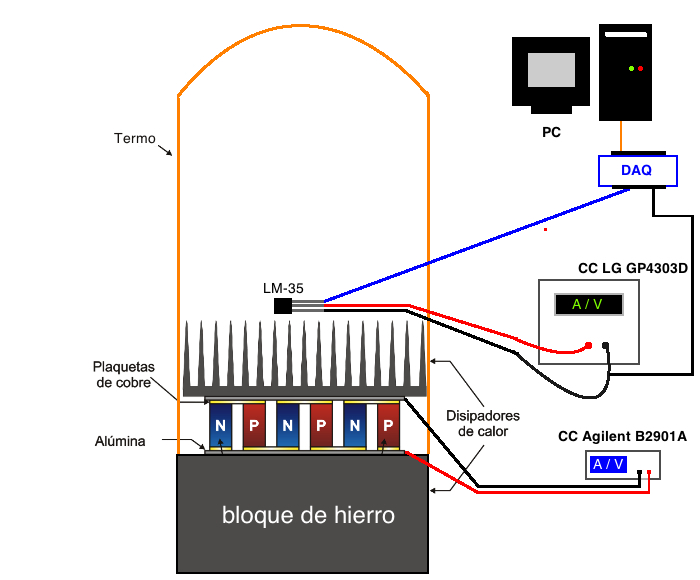
\includegraphics[width=\linewidth]{dispexp2.jpg}
\caption{Esquema del segundo dispositivo experimental utilizado.}
\label{fig:dispexp2}
\end{figure}


%------------------------------------------------
\section{Resultados y an\'alisis}

Lo primero que se pudo observar de forma intuitiva fue que efectivamente, al pasar una corriente por la celda Peltier se produc\'ia una diferencia de temperatura en sus caras, as\'i que se tom\'o registro de dichas temperaturas. En la Figura \ref{fig:temps_C} se puede observar ese registro de y adem\'as, la diferencia de temperaturas en color rojo. Cabe destacar que, como s\'olo nos interesaba observar este fen\'omeno cualitativamente, el gr\'afico se encuentra en grados Celsius mientras que el resto de los resultados los presentaremos en grados Kelvin. Esto se debe a que se puede observar m\'as f\'acilmente que a $\Delta T \approx$ 22,7 \degree C (mismo valor para \degree K), es predominante el efecto Joule y ambas caras de la celda comienzan a calentarse, manteniendo asi una diferencia de temperatura constante. 


\begin{figure}[H]
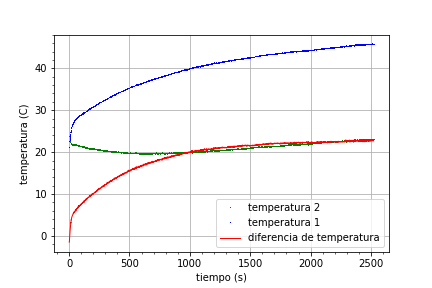
\includegraphics[width=\linewidth]{peltier_temps_C.png}
\caption{Medici\'on de la temperatura mientras ocurre el efecto Peltier. La curva azul es la temperatura de la cara caliente de la celda, mientras que la curva verde es la temperatura de la cara caliente y la curva roja es la diferencia de temperatura.}
\label{fig:temps_C}
\end{figure}


Cuando las caras de la celda llegaron una diferencia de temperatura de $\Delta T \approx$  22,7 \degree C, se quit\'o la fuente de corriente y se observ\'o el efecto Seebeck. El gr\'afico \ref{fig:seebeck} muestra los datos obtenidos de la variaci\'on del voltaje con respecto a la variaci\'on de la diferencia de temperatura entre las caras. Este comportamiento lineal es justamente lo que predijo la aproximaci\'on de la ecuaci\'on (\ref{eq:seebeck2}), en el que la pendiente es el coeficiente de Seebeck. Se realizo un ajuste lineal obteniendo que dicho coeficiente es $\alpha = (6134 \pm 9) * 10^{-6}$ $\frac{V}{\degree K}$.


\begin{figure}[H]
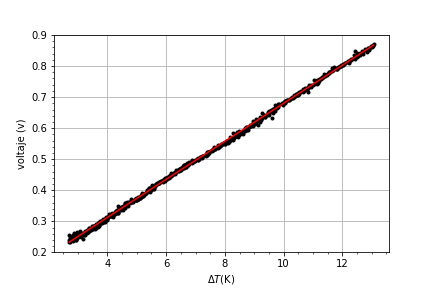
\includegraphics[width=\linewidth]{seebeck_ajuste.png}
\caption{Ajuste lineal de la variaci\'on de la diferencia de potencial con respecto a la variaci\'on de la diferencia de temperaturas en el efecto Seebeck.}
\label{fig:seebeck}
\end{figure}


En la medici\'on del rendimiento detallada en la secci\'on de Dispositivo Experimental se registr\'o la variaci\'on de la diferencia de temperatura con respecto al tiempo, la cual se puede observar en la Figura \ref{fig:joule}. La potencia de la cara fr\'ia $P_{F}$ est\'a dada por la siguiente ecuaci\'on, donde $m_{Al} = (0,025 \pm 0,001)$ g es la masa del disipador de aluminio utilizado y $c_{Al} = 0,89$ $\frac{J}{g \degree K}$ es su calor espec\'ifico.


\begin{equation}
\label{eq:pf}
P_{F} = m_{Al} c_{Al} \frac{\Delta T}{\Delta t}
\end{equation}


Mediante los datos obtenidos para $\alpha$ de la Figura \ref{fig:seebeck}, teniendo en cuenta el \'area de la celda $A = 0,0004 $ $m^{2}$ y la distancia entre las caras $d = 0,003$ m; y bas\'andonos en la ecuaci\'on (\ref{eq:pf}), se realiz\'o un ajuste lineal en el cual se obtuvo la potencia absorbida por la cara fr\'ia, si adem\'as comparamos esta potencia con la potencia entregada a la celda obtenemos, mediante la ecuaci\'on (\ref{eq:rendimiento}), un coeficiente de rendimiento como m\'aquina frigor\'ifica de  $COP = 2,795$. Al comparar este valor con el $COP_{ideal} = \frac{T_{F}}{T_{C}-T_{F}}$, obtenemos un rendimiento del $9.34 \%$ con respecto al rendimiento ideal como maquina frigorifica. 


\begin{figure}[H]
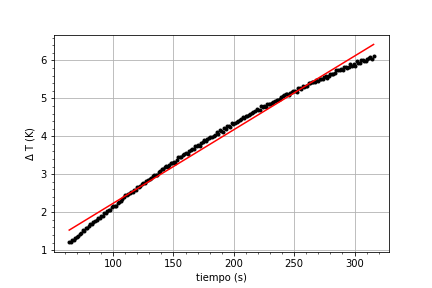
\includegraphics[width=\linewidth]{joule_ajuste.png}
\caption{Ajuste lineal de la variaci\'on de temperatura con respecto al tiempo en la medici\'on del rendimiento como m\'aquina frigor\'ifica.}
\label{fig:joule}
\end{figure}

Para encontrar la resistencia de la placa se utiliz\'o la ecuaci\'on (\ref{eq:potencia}), obteniendo $R = (2,546 \pm 0.081)$ $\Omega$. Finalmente, una vez obtenidos $\alpha$, $R$, $P_{F}$ y adem\'as utilizando los medidas caracteristicas de la celda Peltier, se obtuvo mediante las ecuaciones (\ref{eq:joule}) y (\ref{eq:qcaras}) un valor para la conductividad t\'ermica de  $K = (0,494 \pm 0,110) \frac{W}{m^{2} K}$. Por \'ultimo, la Figura \ref{fig:rendimiento} muestra de forma cualitativa del rendimiento en funci\'on de la variaci\'on de la temperatura. 

\begin{figure}[H]
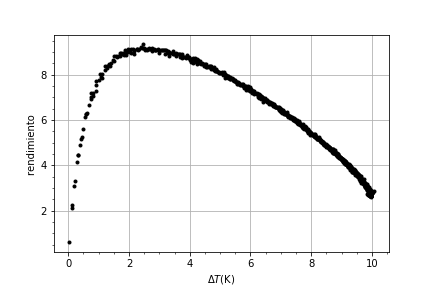
\includegraphics[width=\linewidth]{curva_rendimiento.png}
\caption{Rendimiento de la celda con respecto a la diferencia de temperatura entre sus caras. Se observa que hay un m\'aximo aproximadamente en 9\%. }
\label{fig:rendimiento}
\end{figure}

%------------------------------------------------

\section{Conclusiones}

En este trabajo se realiz\'o la caracterizaci\'on una celda Peltier utilizando dos armados experimentales, el primero para el c\'alculo de su coeficiente de Seebeck $\alpha$ mediante la evoluci\'on de la temperatura en el tiempo, y el segundo para obtener la resistencia $R$, conductividad t\'ermica $K$ y el rendimiento de la celda como m\'aquina frigor\'ifica.\\

Durante la evoluci\'on de la temperatura, la cara caliente aumenta su temperatura de manera continua, mientras que la cara fr\'ia, en un primer momento disminuye su valor hasta llegar a un valor m\'inimo para luego aumentar, evidenciando el efecto Joule. Al alcanzar las caras una $\Delta T \approx$  22,7 \degree C, se quit\'o la fuente de corriente y se observ\'o el efecto Seebeck; para el cual se realizo un ajuste lineal a los datos recolectados ($\Delta V$ en funci\'on de $\Delta T$), obteniendo $\alpha = (6134 \pm 9) * 10^{-6}$ $\frac{V}{\degree K}$. Si bien el coeficiente Seebeck depende de la temperatura; en el intervalo de tiempo trabajado ($\approx$ 16 min) se comporta de manera constante.\\	

Para la medici\'on del rendimiento se registr\'o la variaci\'on de la diferencia de temperatura con respecto al tiempo. Se obtuvo ademas la potencia de la cara fr\'ia $P_{F}$ en funcion de estos par\'ametros y la potencia de la celda como el producto entre la corriente y el voltaje entregado por el generador de corriente continua, obteniendo un coeficiente de rendimiento como m\'aquina frigor\'ifica de $COP = 2,795$, es decir, un $9.34 \%$ del rendimiento de una maquina ideal como maquina frigorifica.\\

Por \'ultimo, con los datos obtenidos y utilizando la ecuaci\'on (\ref{eq:potencia}) se obtuvo la resistencia de la celda $R = (2,546 \pm 0.081)$ $\Omega$. Utilizando este valor y los hallados para $\alpha$, $P_{F}$ y las medidas de la celda (\'area $A$ y distancia entre caras $d$), se encontr\'o el valor para la conductividad t\'ermica de  $K = (0,494 \pm 0,110) \frac{W}{m^{2} K}$, resultando un poco m\'as baja que la del agua; comparable con materiales como ladrillo refractario o mica.

%----------------------------------------------------------------------------------------
%	REFERENCE LIST
%----------------------------------------------------------------------------------------
\newpage
\begin{thebibliography}{99} % Bibliography - this is intentionally simple in this template


[1] -- [6] http://materias.df.uba.ar/labo4Ba2016c1/files
           /2016/03/Guia\_L4\_Peltier.pdf
 
\end{thebibliography}


%----------------------------------------------------------------------------------------

\end{document}